%%%%%%%%%%%%%%%%%%%%%%%%%%%%%%%%%%%%%%%%%%%%%%%%%%%%%
%%% Task 3 %%%%%%%%%%%%%%%%%%%%%%%%%%%%%%%%%%%%%%%%%%
%%%%%%%%%%%%%%%%%%%%%%%%%%%%%%%%%%%%%%%%%%%%%%%%%%%%%
\task{Transformer}

%%%%%%%%%%%%%%%%%%%%%%%%%%%%%%%%%%%%%%%%%%%%%%
\taskGerman{Transformator}
% Frage 5: Welche idealisierte sekundäre Ausgangsspannung ergibt sich, wenn der Transformator zum Spartransformator umgewickelt wird? Welcher primäre Kurzschlusstrom ergibt sich nun, falls sekundär kurzgeschlossen wird? 


\subtask{Draw and label the T-type equivalent circuit diagram of a single phase transformer.}{1}
\subtaskGerman{Zeichnen und beschriften Sie das T-Ersatzschaltbild eines einphasigen Transformators.}

\begin{solutionblock}
    \begin{solutionfigure}[ht]
    \centering
    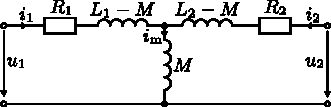
\includegraphics[width=0.6\textwidth]{fig/Transformer_T_ECD.pdf}
    \caption{T-type equivalent circuit diagram of a single phase transformer}
    \label{fig:Transformer_T_ECD}
    \end{solutionfigure}
\end{solutionblock}

\subtask{The primary side has $N_1 = 23$ and the secondary side has $N_2=10$ turns. For $\underline{U}_1 = \SI{230}{\volt}$, which secondary voltage $U_2$ would you expect for an unloaded, idealized transformer?}{1}
\subtaskGerman{Die Primärwicklung hat $N_1 = 23$ und die Sekundärwicklung hat $N_2=10$ Windungen. Welche Sekundärspannung $U_2$ würden Sie bei $\underline{U}_1 = \SI{230}{\volt}$ für einen unbelasteten, idealisierten Transformator erwarten?}

\begin{solutionblock}
    For the described idealized case the voltage transformation ratio is
    $$
    U_2 = \frac{U_1}{\"u} = U_1 \frac{N_2}{N_1} = \SI{230}{\volt} \cdot \frac{10}{23} = \SI{100}{\volt}. 
    $$
\end{solutionblock}

\subtask{Which actual voltage $U_2$ is to be expected if the transformer is loaded with $\underline{I}_2=\SI{-10}{\ampere}$ considering the following parameters: $R_1 \approx \SI{0}{\ohm}$, $R_2 = \SI{0.1}{\ohm}$, $M = \SI{0.42}{\henry}$, $L_1 =\SI{1}{\henry}$, $L_2 =\SI{0.17}{\henry}$?}{2}
\subtaskGerman{Welche tatsächliche Spannung $U_2$ ist zu erwarten, wenn der Transformator mit $\underline{I}_2=\SI{-10}{\ampere}$ belastet wird und folgende Parameter aufweist: $R_1 \approx \SI{0}{\ohm}$, $R_2 = \SI{0,1}{\ohm}$, $M = \SI{0,42}{\henry}$, $L_1 =\SI{1}{\henry}$, $L_2 =\SI{0,17}{\henry}$?}

\begin{solutionblock}
    The steady-state complex current and voltage phasors of the transformer are:
    \begin{align*}
			 \begin{bmatrix} \underline{U}_1 \\ \underline{U}_2 \end{bmatrix} =  \begin{bmatrix} R_1 + \mathrm{j} \omega_\mathrm{el} L_1 & \mathrm{j} \omega_\mathrm{el} M \\ \mathrm{j} \omega_\mathrm{el} M & R_2 + \mathrm{j}\omega_\mathrm{el} L_2 \end{bmatrix} \begin{bmatrix} \underline{I}_1 \\ \underline{I}_2 \end{bmatrix}.
		\end{align*}
    Considering $R_1\approx 0$ and rearranging the first line yields
    $$
    \underline{I}_1 = \frac{\underline{U}_1 - \mathrm{j} \omega_\mathrm{el} M \underline{I}_2}{\mathrm{j} \omega_\mathrm{el} L_1}. 
    $$
    Inserting that into the second line
    $$
    \underline{U}_2 = \mathrm{j} \omega_\mathrm{el} M \underline{I}_1 + (R_2 + \mathrm{j}\omega_\mathrm{el} L_2)\underline{I}_2 
    $$
    delivers
    $$
    \underline{U}_2 = \frac{M}{L_1}\underline{U}_1 + \left[R_2 + \mathrm{j}\omega_\mathrm{el}\left( L_2-\frac{M^2}{L_1}\right)\right]\underline{I}_2.
    $$
    Inserting the given parameter values yields
    \begin{align*}
    \underline{U}_2 &= \frac{\SI{0.42}{\henry}}{\SI{1}{\henry}}\cdot\SI{230}{\volt} + \left[\SI{0.1}{\ohm} + \mathrm{j}\SI{314.16}{\per\second}\left( \SI{0.17}{\henry}-\frac{(\SI{0.42}{\henry})^2}{\SI{1}{\henry}}\right)\right]\cdot(\SI{-10}{\ampere})\\
     &= \SI{95.6}{\volt} - \mathrm{j} \SI{20.11}{\volt}
    \end{align*}
    finally leading to
    $$
    U_2 = \SI{97.69}{\volt}.
    $$
\end{solutionblock}

\subtask{Which primary prospective short-circuit current $I_{1,\mathrm{psc}}$ occurs if the secondary side is short-circuited?}{2}
\subtaskGerman{Welcher primäre Dauerkurzschlussstrom $I_{1,\mathrm{psc}}$ tritt auf, wenn die Sekundärseite kurzgeschlossen wird?}

\begin{solutionblock}
    The short circuit relates to $U_2=0$ leading to
    $$
    0 = \mathrm{j} \omega_\mathrm{el} M \underline{I}_1 + (R_2 + \mathrm{j}\omega_\mathrm{el} L_2)\underline{I}_2 \quad \Leftrightarrow \quad  \underline{I}_2 = \frac{-\mathrm{j} \omega_\mathrm{el} M }{R_2 + \mathrm{j}\omega_\mathrm{el} L_2} \underline{I}_1.
    $$
    Inserting into the primary voltage equations yields
    $$
    \underline{I}_1 = \frac{1}{\mathrm{j} \omega_\mathrm{el} L_1}\underline{U}_1 + \frac{M}{L_1} \frac{\mathrm{j} \omega_\mathrm{el} M }{R_2 + \mathrm{j}\omega_\mathrm{el} L_2} \underline{I}_1. 
    $$
    Solving for $\underline{I}_1$
    $$
    \underline{I}_1 = \left(1 - \frac{M}{L_1} \frac{\mathrm{j} \omega_\mathrm{el} M }{R_2 + \mathrm{j}\omega_\mathrm{el} L_2}\right)^{-1}\frac{1}{\mathrm{j} \omega_\mathrm{el} L_1}\underline{U}_1
    $$
    and some rewriting
    \begin{align*}
        \underline{I}_1 
        & =\left(\frac{L_1 R_2 +\mathrm{j} \omega_\mathrm{el} (L_1 L_2-M^2)}{L_1(R_2 + \mathrm{j}\omega_\mathrm{el} L_2)}\right)^{-1}\frac{1}{\mathrm{j} \omega_\mathrm{el} L_1}\underline{U}_1\\
        & =\left(\frac{(R_2 + \mathrm{j}\omega_\mathrm{el} L_2)}{L_1 R_2 +\mathrm{j} \omega_\mathrm{el} (L_1 L_2 -M^2)}\right)\frac{1}{\mathrm{j} \omega_\mathrm{el}}\underline{U}_1\\ 
        & =\left(\frac{(R_2 + \mathrm{j}\omega_\mathrm{el} L_2)}{L_1 R_2\mathrm{j}\omega_\mathrm{el} - \omega_\mathrm{el}^2 (L_1 L_2 -M^2)}\right)\underline{U}_1 \\
        & =-\left(\frac{(R_2 + \mathrm{j}\omega_\mathrm{el} L_2)(L_1 R_2\mathrm{j}\omega_\mathrm{el} + \omega_\mathrm{el}^2 (L_1 L_2 -M^2))}{(L_1 R_2\omega_\mathrm{el})^2 + \omega_\mathrm{el}^4 (L_1 L_2 -M^2)^2}\right)\underline{U}_1
    \end{align*}
finally leads to
\begin{align*}
\underline{I}_{1,\mathrm{psc}} &= (\SI{4.4\cdot 10^{-3}}{\per\ohm} + \mathrm{j}\cdot\SI{84.3\cdot 10^{-3}}{\per\ohm}) \cdot \SI{230}{\volt}\\
                              &= \SI{1.0}{\ampere} + \mathrm{j}\cdot\SI{19.40}{\ampere},
\end{align*}     
that is, is $I_{1,\mathrm{psc}} = \SI{19.42}{\ampere}$.
\end{solutionblock}

\subtask{What idealized secondary output voltage results in the unloaded case when the transformer is reconfigured as an autotransformer connecting the terminals 1.1 and 2.2?}{1}
\subtaskGerman{Welche idealisierte sekundäre Ausgangsspannung ergibt sich im unbelasteten Fall, wenn der Transformator zum Spartransformator mittels Verbinden der Klemmen 1.1 und 2.2 abgewandelt wird?}
\begin{figure}[ht]
    \centering
    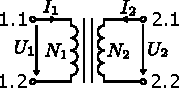
\includegraphics[width=0.3\textwidth]{fig/Autotransformer_connection.pdf}
    \caption{Transformer connection nomenclature}
    \label{fig:Autotransformer_connection}
\end{figure}

\begin{solutionblock}
The described case refers to a step-up autotransformer, cf. \autoref{fig:Autotransformer_step_up}. Hence, the new secondary output voltage is $U_\mathrm{at,out} = U_1 + U_2 = \SI{330}{\volt}.$
    \begin{solutionfigure}[ht]
    \centering
    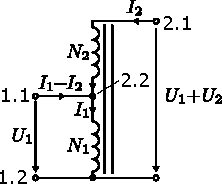
\includegraphics[width=0.3\textwidth]{fig/Autotransformer_step_up.pdf}
    \caption{Step-up autotransformer}
    \label{fig:Autotransformer_step_up}
\end{solutionfigure}
\end{solutionblock}

\subtask{Calculate the change in primary current in the event of a short circuit on the secondary side of the autotransformer compared to the original galvanically isolated transformer.}{1}
\subtaskGerman{Beziffern Sie die Veränderung des Primärstroms im Fall eines Kurzschlusses auf der Sekundärseite des Spartransformators im Vergleich zum ursprünglichen galvanisch getrennten Transformator.}

\begin{solutionblock}
    Due to the reconfiguration the effective short-circuit impedance is decreased and the resulting primary short-circuit current is increased:
    $$
    I_{1,\mathrm{at,psc}} = \left(1+ \frac{N_1}{N_2}\right) I_{1,\mathrm{psc}} = (1+2.3) \cdot \SI{19.42}{\ampere} = \SI{64.09}{\ampere}. 
    $$
    The primary short-circuit current is $3.3$ times higher than for the original transformer configuration. 
\end{solutionblock}
